\section{Contexte du projet}

\subsection{Présentation du projet et ces objectives}

\begin{figure}[h!]  
  \centering
    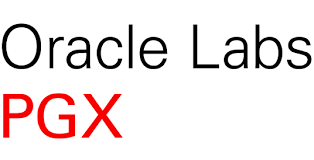
\includegraphics[width=0.7\textwidth]{chapitre1/Figures/PGX-logo.png}
\end{figure}

Les bases de données de graphes, est parmi les derniers outils nés pour les data scientistes, et data analystes après le BigData il y a quelques années. Ils ont vu le jour pour résoudre des problèmes d’extraction et de traitement des données précédemment difficiles à approcher avec les outils déjà existants. Vous pouvez certainement faire le même type d'analyse qu'une base de données de graphes vous permet de faire sur votre base de données relationnelle. Mais vous devrez écrire des tonnes de code et il sera probablement assez mal exécuté.\\
Selon le classement [b.12] Gartner en 2019, les outils de traitements et analyse des graphes constitue la tendance numéro 5 dans le domaine d’analyse des données et explique : \\
« L'application du traitement des graphes et des SGBD de graphes connaîtra une croissance annuelle de 100\% jusqu'en 2022 afin d'accélérer continuellement la préparation des données et de permettre une science des données plus complexe et plus adaptative. \\
Les entrepôts de données des graphes peuvent efficacement modéliser, explorer et interroger des données avec des interrelations complexes. Mais le besoin de compétences spécialisées a limité leur adoption jusqu'à présent.\\
L'analyse des graphes se développera dans les prochaines années en raison de la nécessité de poser des questions complexes à travers des données complexes, ce qui n'est pas toujours pratique ou même possible à l'échelle en utilisant des requêtes SQL »\\
Oracle a rejoint ce mouvement avec sa solution de graphes de propriétés : PGX, l'acronyme de Parallel Graph AnalytiX. PGX lui-même se manifeste sous deux formes, PGX.SM (PGX Shared Memory) et PGX.D (PGX Distributed), à chacun ces avantages. Cette flexibilité permet à Oracle d’être un grand compétiteur.\\
GX peut être un outil d’analyse des graphes autonome, et il est aussi le cerveau des implémentations de graphe qu'Oracle utilise dans divers outils comme FCC Studio, Data studio et autres. Cet outil qui effectue des opérations sur les graphes en mémoire, mais ne fournit pas de stockage direct (Figure 2). Le stockage (lecture et écriture) est fourni par des solutions externes comme les fichiers du système (filesystem), SQL (database), NoSQL, Spark et HDFS.\\

\begin{figure}[h!]  
  \centering
    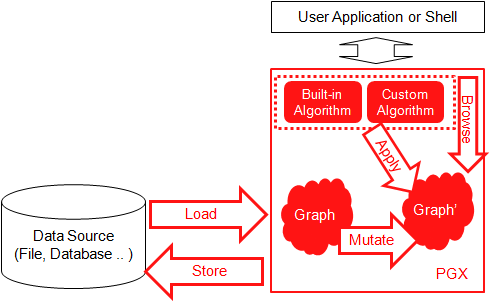
\includegraphics[width=0.8\textwidth]{chapitre1/Figures/pgx_overview.png}
  \caption{Architecture PGX}
\end{figure}

\subsection{Compétiteurs de PGX}

Orcale n’est pas l’unique utile de traitement des graphes sur le marché, Il y a plusieurs compétiteurs industriels ainsi que ceux académique. Dans la suite de cette section je vais montrer quelques comparaisons entre PGX et d’autres systémies.\\
\begin{itemize}
\item PGX offre plus des facilités pour les analystes pour augmenter la productivité comme montre le tableau suivant :
\begin{table}[H]  
  \centering
    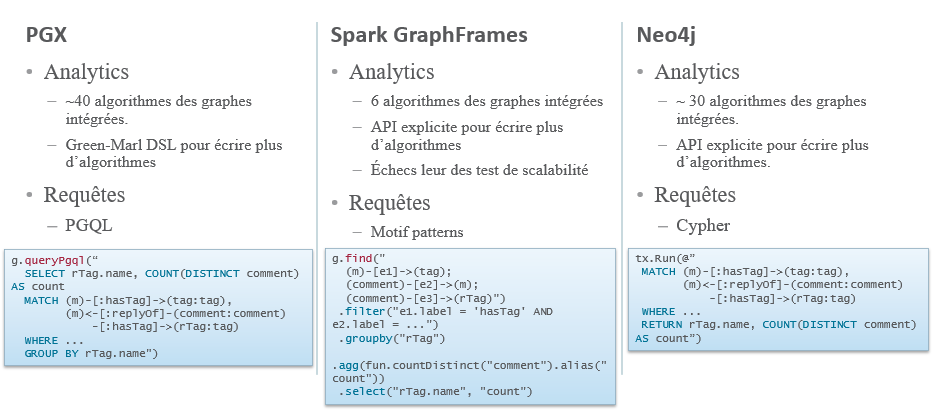
\includegraphics[width=1.15\textwidth]{chapitre1/Figures/FonctionalitesPGX.png}
  \caption{Comparaison des fonctionnalités entre PGX, GraphFrames et Neo4j [a.4]}
\end{table}

\item PGX offre une meilleure performance par rapport aux autres systèmes.

\begin{table}[H]  
  \centering
    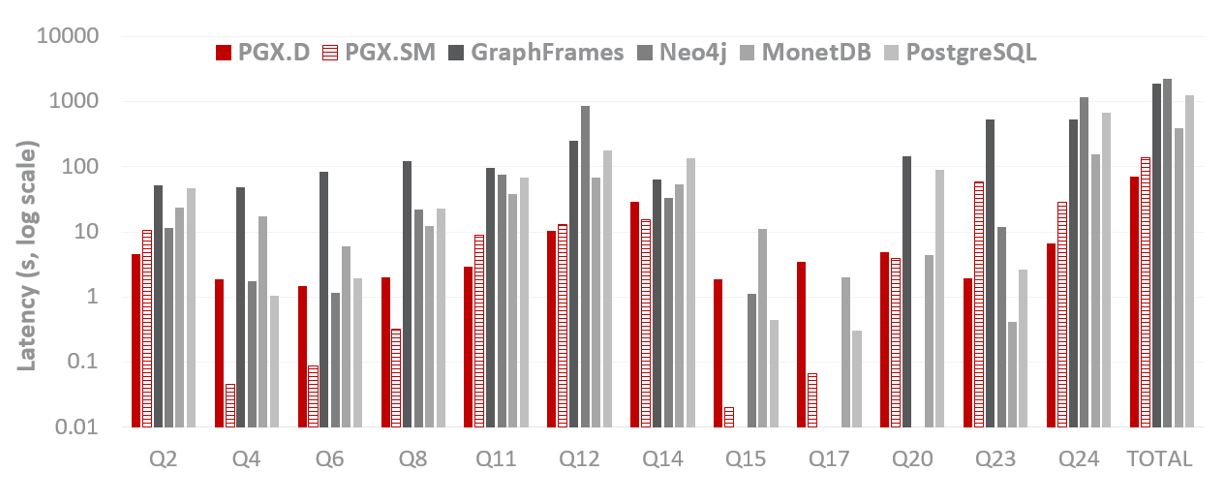
\includegraphics[width=1.15\textwidth]{chapitre1/Figures/BenchmarkLDBC.png}
  \caption{Benchmark LDBC; 8 machines pour PGX.D et GraphFrames}
\end{table}
\end{itemize}

\subsection{Conduite du projet}
La conduite de projet était cadrée par l’approche agile SCRUM, elle est l’une des méthodologies les plus utilisées dans le développement logiciel. SCRUM étant une approche qui suit la méthodologie agile, implique la participation active du client tout au long du projet.\\
L’approche SCRUM et choisie vue ces avantages, à citer la diminution de la possibilité de livrer un projet complet qui ne répond pas ou besoins du client, puisque celui-ci ca toujours une vision imprécise qui s’améliore au cours du temps.\\
SCRUM répondre au besoin et aux exigences du client en termes de qualité et de fonctionnement, par ça flexibilité et adaptabilité aux évolutions éventuelles des besoins métiers. La démarche à choisir devrait également assurer l’implication du client dans le projet, et ceci en livrant à la fin de chaque itération un produit fonctionnel et testable.\\
Le feedback devra être pris en considération dans les versions suivantes de l’itération.\\

\begin{figure}[h!]  
  \centering
    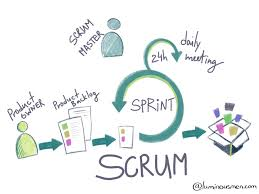
\includegraphics[width=0.7\textwidth]{chapitre1/Figures/SCRUM.jpg}
  \caption{Processus SCRUM}
\end{figure}

Pour bien suivre le projet et implémenter la méthode SCRUM de manière efficace, L’équipe PGX opte pour les solutions ATLASSIAN suivantes :
\begin{itemize}
\item Confluence : Pour documenter, discuter et partager tout information lié ou projet comme la conception, et l’analyse des nouvelles fonctionnalités. 
\item JIRA : Pour affecter des tâches à chaque membre de l’équipe, suivre le backlog, et l’état du sprint.
\item BitBucket : Une alternative a github et gitlab, qui implémente le protocole GIT la collaboration efficace des équipes des tous les tailles.
\end{itemize}
Ces trois solutions sont interdépendantes et permettent d’automatiser certaines tâches, comme la modification de l’état du ticket en JIRA selon l’état de celle-ci dans BitBucket.\\

\subsection{Diagramme de Gante}
\begin{figure}[h!]  
  \centering
    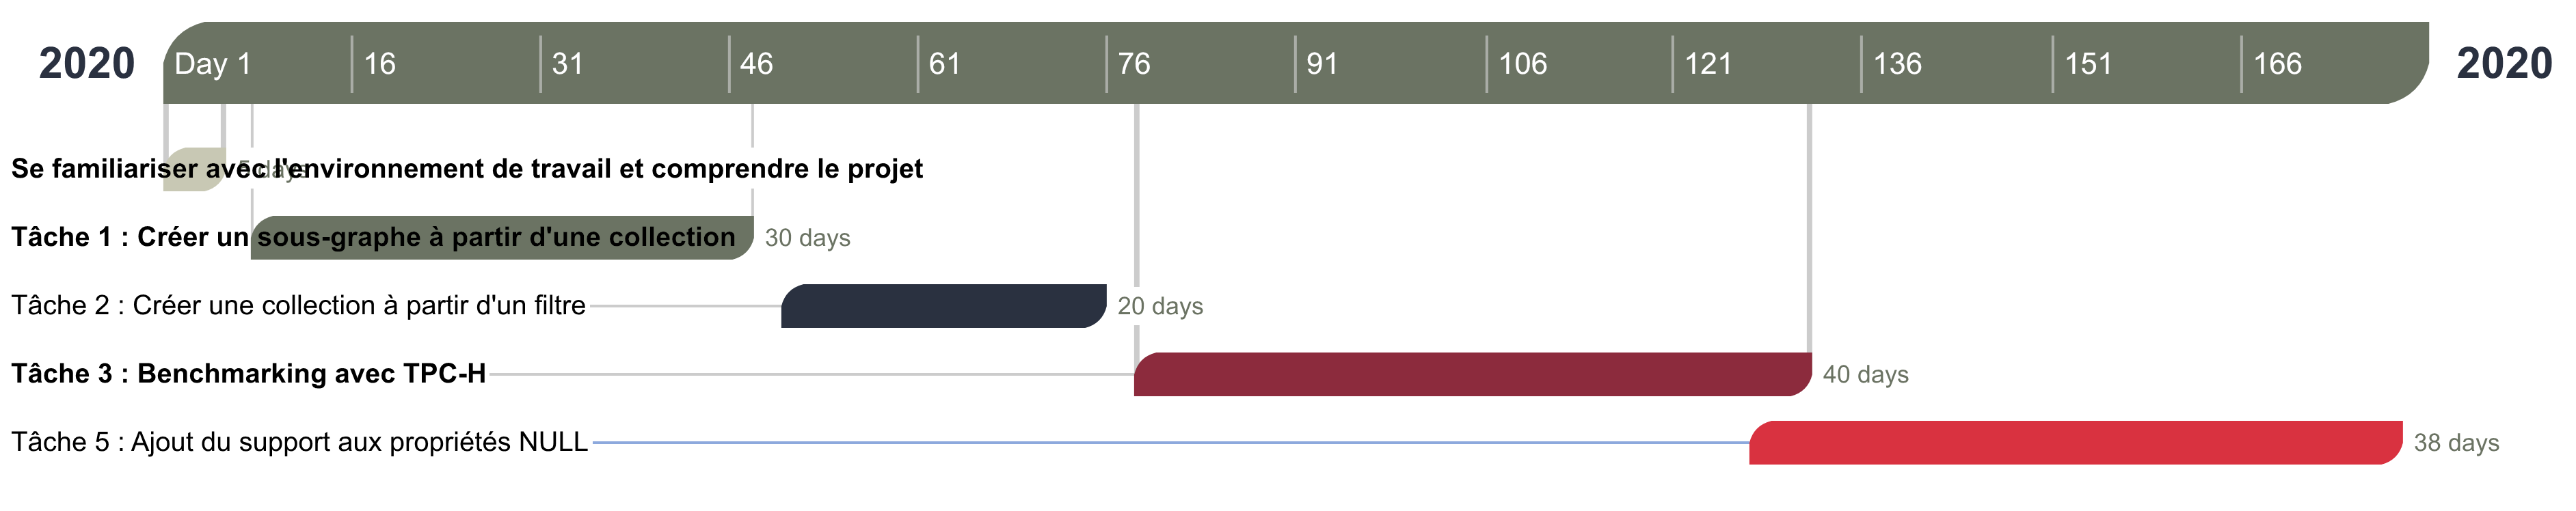
\includegraphics[width=1.2\textwidth]{chapitre1/Figures/PlanningRoadmap.png}
  \caption{Diagramme de Gante de déroulement du stage}
\end{figure}